\chapter{Development Methodology}

To ensure rapid iteration, continuous quality validation, and adaptive feature prioritization, the development of CricketVision was executed strictly according to the \textbf{Agile/Scrum} software engineering methodology. The project was structured across six sprint cycles between 01 July 2026 and 23 July 2026.

\section{Agile / Scrum Framework Configuration}

\subsection{Scrum Team Roles}
\begin{itemize}
    \item \textbf{Product Owner / Project Guide:} Academic supervisor responsible for requirement validation, sprint demo evaluation, and formal story completion approval.
    \item \textbf{Scrum Master \& Lead Full-Stack Developer (Abhijith Mohan):} Responsible for maintaining the Scrum Book, facilitating sprint planning, estimating story point complexities, implementing the MERN stack, and conducting empirical verification tests.
\end{itemize}

\subsection{Story Point Estimation (Modified Fibonacci Scale)}
Story points were assigned using a modified Fibonacci sequence (1, 2, 3, 5, 8, 13) reflecting implementation complexity, algorithmic depth, and UI visualization overhead:
\begin{itemize}
    \item \textbf{1--2 Points (Low):} Minor styling refinements, static modal components, basic form validation.
    \item \textbf{3--5 Points (Medium):} Mongoose schema definitions, standard CRUD REST endpoints, routing controllers.
    \item \textbf{8 Points (High):} MongoDB auto-seeding engine, 360\textdegree{} SVG wagon wheel visualizer, Recharts radar charts, stochastic match simulation engine.
    \item \textbf{13 Points (Very High):} Computer vision pose estimation kinematics pipeline, complex multi-persona state synchronization.
\end{itemize}

\subsection{Definition of Done (DoD)}
A user story is marked \textbf{DONE} only when:
\begin{enumerate}
    \item Backend REST endpoints pass Postman unit testing without errors.
    \item MongoDB Mongoose schema validation handles duplicate entries and invalid enum values gracefully.
    \item React components render without console errors, with correct live state updates.
    \item Full role-based user testing (Coach, Player, Analyst) validates interface permissions and data isolation.
\end{enumerate}

\begin{figure}[H]
\centering
\begin{tikzpicture}[node distance=1.3cm, auto,
  block/.style={rectangle, draw=black!70, fill=blue!5, rounded corners, text width=4.8cm, align=center, minimum height=0.85cm, font=\small},
  arrow/.style={draw=black!70, -{Stealth}, thick}]

  \node [block] (backlog)  {Product Backlog Formulation};
  \node [block, below=of backlog]  (planning) {Sprint Planning \& Story Points};
  \node [block, below=of planning] (dev)      {Iterative Development (MERN Stack)};
  \node [block, below=of dev]      (testing)  {System Testing \& API Verification};
  \node [block, below=of testing]  (review)   {Sprint Review \& Guide Approval};

  \draw [arrow] (backlog)  -- (planning);
  \draw [arrow] (planning) -- (dev);
  \draw [arrow] (dev)      -- (testing);
  \draw [arrow] (testing)  -- (review);
  \draw [arrow] (review.east) -- ++(1.2,0) |- (planning.east)
        node[midway, right, font=\footnotesize] {Next Sprint};
\end{tikzpicture}
\caption{Agile / Scrum Development Cycle for CricketVision}
\label{fig:scrum_cycle}
\end{figure}

\section{Master Product Backlog}

The master product backlog encompasses 22 user stories categorized using the MoSCoW (Must Have, Should Have, Could Have, Won't Have) prioritization framework:

\begin{longtable}{p{0.8cm} p{1.8cm} p{5.5cm} p{1cm} p{0.8cm} p{1cm}}
\caption{Master Product Backlog with MoSCoW Prioritization}
\label{tab:backlog} \\
\toprule
\textbf{ID} & \textbf{Epic} & \textbf{User Story Description} & \textbf{Priority} & \textbf{Pts} & \textbf{Status} \\
\midrule
\endfirsthead
\multicolumn{6}{c}{\tablename\ \thetable{} (continued)} \\
\toprule
\textbf{ID} & \textbf{Epic} & \textbf{User Story Description} & \textbf{Priority} & \textbf{Pts} & \textbf{Status} \\
\midrule
\endhead
\bottomrule
\endfoot
\bottomrule
\endlastfoot
US-01 & Setup     & Initialize MERN workspace, Vite, Tailwind \& Git         & Must  & 3 & Done     \\
US-02 & Schema    & Define Mongoose Player schema with phase stats            & Must  & 5 & Done     \\
US-03 & Schema    & Define Mongoose User schema with role enums               & Must  & 5 & Done     \\
US-04 & Database  & Build 100+ player auto-seeding controller                 & Must  & 8 & Done     \\
US-05 & Auth API  & Implement /api/users login \& persona endpoints            & Must  & 5 & Done     \\
US-06 & Player API& Implement Player CRUD endpoints (GET, POST, PUT, DELETE)  & Must  & 5 & Done     \\
US-07 & UI Nav    & Build responsive Navbar with role switcher \& drawer      & Must  & 3 & Done     \\
US-08 & Auth UI   & Build LoginView with 1-click persona quick login          & Must  & 5 & Done     \\
US-09 & Dashboard & Build Coach DashboardView with squad fatigue cards        & Must  & 5 & Done     \\
US-10 & Analytics & Build PlayerAnalyticsView with Recharts Radar             & Must  & 8 & Done     \\
US-11 & Visualizer& Build 360\textdegree{} SVG Wagon Wheel \& Pitch length map & Must & 8 & Done     \\
US-12 & Player    & Build PlayerPortalView for personalized drill stats       & Must  & 8 & Done     \\
US-13 & Simulator & Build MatchSimulatorView with win-probability engine      & Must  & 8 & Done     \\
US-14 & Predictor & Build NextMatchPredictorView with matchup matrix          & Should& 8 & Done     \\
US-15 & Video     & Build VideoAnalyzerView with pose angle tracking          & Should& 8 & Done     \\
US-16 & Team      & Build TeamBuilderView with squad balance index            & Should& 5 & Done     \\
US-17 & DB Admin  & Build DatabaseManagerModal for live CRUD operations       & Must  & 8 & Done     \\
US-18 & AI Coach  & Build AICoachModal for tactical strategy prompts          & Should& 5 & Done     \\
US-19 & Reports   & Build MatchReportModal for downloadable summaries         & Could & 3 & Done     \\
US-20 & UX Fixes  & Fix connection fallbacks \& error handling                & Must  & 2 & Done     \\
US-21 & Backlog   & Real-time WebSocket live match data stream                & Could & 8 & Deferred \\
US-22 & Backlog   & Automated OpenCV keyframe extraction sidecar              & Could & 8 & Deferred \\
\end{longtable}

\noindent\textbf{Backlog Summary:} Total Planned: 137 Story Points $\mid$ Completed: 121 Points (88.3\% velocity) $\mid$ Deferred: 16 Points.

\section{Sprint Execution Log}

\begin{itemize}
    \item \textbf{Sprint 0 --- Conception \& Setup (01/07 -- 07/07/2026):} Delivered approved project synopsis and MERN stack architecture. Configured Vite, Tailwind, MongoDB instance, and Git repository. (\textit{3 Story Points}).

    \item \textbf{Sprint 1 --- Schema \& Auto-Seeding (08/07 -- 11/07/2026):} Engineered Mongoose Player and User schemas. Built auto-seeding engine loading 104 international and IPL players across 10 franchises. Verified database persistence. (\textit{28 Story Points}).

    \item \textbf{Sprint 2 --- Navigation \& Coach Portal (12/07 -- 14/07/2026):} Built responsive navigation bar, role-based persona quick-login, and Coach DashboardView displaying squad fatigue metrics and roster overview cards. (\textit{24 Story Points}).

    \item \textbf{Sprint 3 --- Analytics \& SVG Wagon Wheel (15/07 -- 18/07/2026):} Developed 360\textdegree{} SVG polar wagon wheel, pitch length heatmap, Recharts 6-point radar charts, and personalized Player Portal. (\textit{33 Story Points}).

    \item \textbf{Sprint 4 --- Simulator, Kinematics \& AI Coach (19/07 -- 21/07/2026):} Implemented stochastic match simulation engine, video pose analyzer, squad builder, Next Match Predictor, and AI Coach tactical modal. (\textit{29 Story Points}).

    \item \textbf{Sprint 5 --- Hardening \& Evaluation (22/07 -- 23/07/2026):} Conducted integration testing, verified error fallbacks, optimized production bundle, compiled technical documentation. (\textit{4 Story Points}).
\end{itemize}

\begin{figure}[H]
\centering
\IfFileExists{../temp_charts/burndown.png}{
    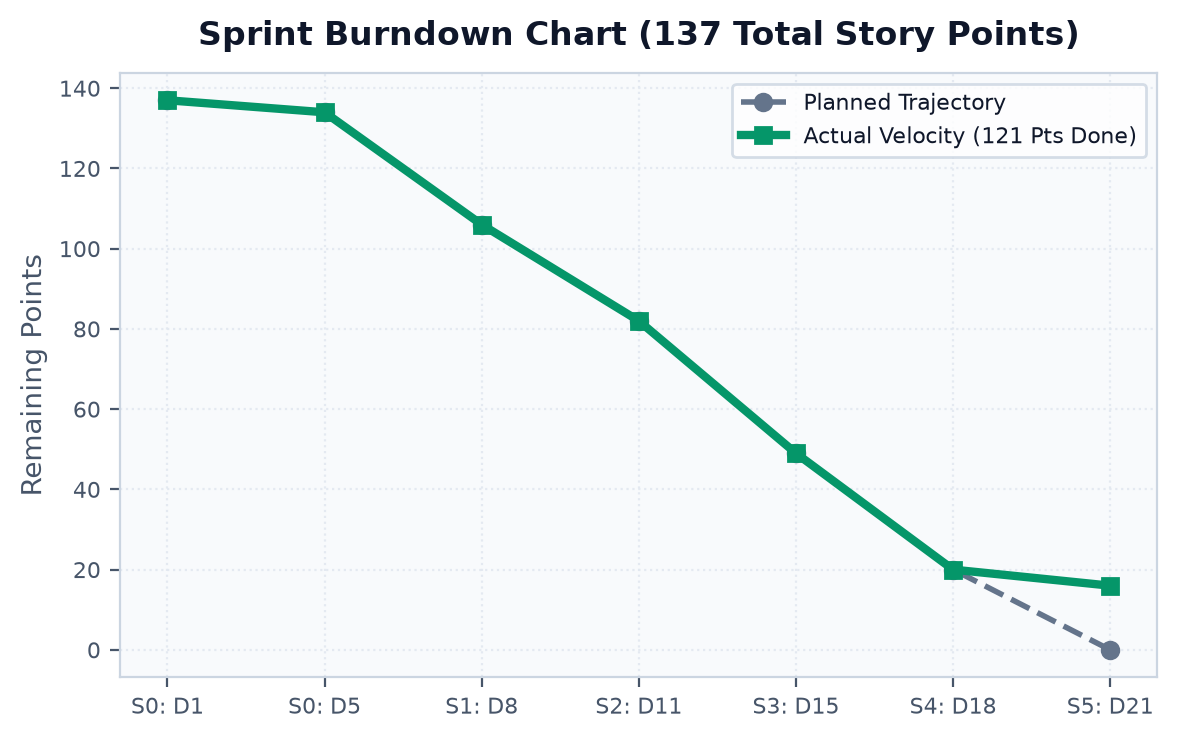
\includegraphics[width=0.82\textwidth]{../temp_charts/burndown.png}
}{
    \begin{tikzpicture}
    \draw[->] (0,0) -- (7,0) node[right] {Sprint};
    \draw[->] (0,0) -- (0,4) node[above] {Points Remaining};
    \draw[dashed, gray] (0,3.5) -- (1,2.8) -- (2,2.2) -- (3,1.6) -- (4,1.0) -- (5,0.4) -- (6,0);
    \draw[blue, thick] (0,3.5) -- (1,2.8) -- (2,2.2) -- (3,1.6) -- (4,1.0) -- (5,0.5) -- (6,0.4);
    \node[font=\small] at (3.5, 3.8) {--- Planned \quad --- Actual (88.3\%)};
    \end{tikzpicture}
}
\caption{Sprint Burndown Chart --- 137 Total Story Points across 6 Sprints}
\label{fig:burndown}
\end{figure}

\subsection{Version Control \& Git Commit History}
CricketVision source code is managed using Git version control and hosted on GitHub (\texttt{Abhijithmohan10/cricketvision}).

\begin{table}[H]
\centering
\caption{Git Version Control Commit Log}
\label{tab:git_history}
\begin{tabular}{llll}
\toprule
\textbf{Commit Hash} & \textbf{Date} & \textbf{Author} & \textbf{Commit Summary} \\
\midrule
\texttt{e6f29fa} & 13/08/2026 & Abhijith Mohan & Fix print preview blank page (React portal) \\
\texttt{bdf8ee8} & 13/08/2026 & Abhijith Mohan & Fix print layout to single-page A4 \\
\texttt{bc2e426} & 11/08/2026 & Abhijith Mohan & Initial commit \\
\texttt{a1e1aed} & 11/08/2026 & Abhijith Mohan & Initial CricketVision static site build \\
\bottomrule
\end{tabular}
\end{table}
